% figures/state/cant_interpretation.tex
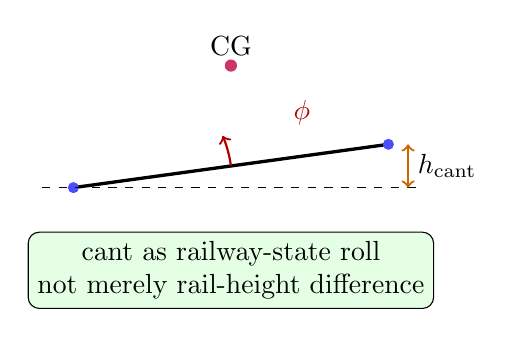
\begin{tikzpicture}[
  x=1cm,y=1cm,
  box/.style={draw, rounded corners, align=center, minimum width=3.5cm, minimum height=0.8cm},
  arrow/.style={->, thick}
]
\coordinate (L) at (-2,0);
\coordinate (R) at (2,0.55);
\draw[very thick] (L) -- (R);
\fill[blue!70] (L) circle (2pt);
\fill[blue!70] (R) circle (2pt);

\draw[dashed] (-2.4,0) -- (2.4,0);
\draw[<->, thick, orange!80!black] (2.25,0) -- (2.25,0.55);
\node[right] at (2.25,0.28) {$h_{\mathrm{cant}}$};

\draw[->, thick, red!70!black] (0,0.28) arc[start angle=8,end angle=23,radius=1.5];
\node[red!70!black] at (0.9,0.95) {$\phi$};

\coordinate (CG) at (0,1.55);
\fill[purple!80] (CG) circle (2.2pt);
\node[above] at (CG) {CG};

\node[box, fill=green!10] at (0,-1.05) {cant as railway-state roll\\not merely rail-height difference};
\end{tikzpicture}
